\chapter{Entscheiden}
\label{chap:decide}
In diesem Kapitel werden Entscheidungen und dessen Begründungen dokumentiert. \newline
Da diese PA ein Plugin für bereits etablierte Software ist, gibt es, vor allem bezüglich des Tech-Stacks, nicht viel zu
entscheiden. Wie die zweite Software-Design Anforderung besagt: \enquote{Das Plugin soll sich an die Coding-Guidelines von
Redmine halten...} \newline
Für das Bewerten wurden alle Optionen vorgelegt und kurz beschrieben. Dann wurde mit einer Entscheidungsmatrix
bewertet und gewählt.

\section{Bewertungen}
\subsection{Entity-Relationship-Diagram}
\subsubsection{Option 1: Mehrere Entitäten}
Die erste Option, wie auf Grafik \ref{fig:erd_multiple} zu sehen, ist, dass für Deployments und Pull-Requests
eigene Entitäten erstellt werden, welche beide direkt mit den Issues verbunden sind. \newline
Die Vorteile dieser Option sind beispielsweise, dass die Komplexität der Datenstruktur gering ist. Es ist einfach zu
implementieren und eventuellen späteren Entwicklern zu erklären. \newline
Ein grosser Nachteil dieser Datenstruktur ist, dass wahrscheinlich zwei separate Controller erstellt werden müssen, was
die Codebase unnötig vergrössert (aber nicht unbedingt Komplexität hinzufügt).

\subsubsection{Option 2: Inheritance}
Die zweite Option, wie auf Grafik \ref{fig:erd_inheritance} zu sehen, ist, dass für Deployments und Pull-Requests nur
Child-Entitäten erstellt werden, welche beide von einer gemeinsamen Entität erben. \newline
Der grösste Vorteil dieser Option ist, dass die Vererbung die Codebase vereinfachen kann, falls richtig implementiert.
\newline
Nachteile sind, dass die Komplexität der Datenstruktur massiv erhöht wird. Vererbung ist in Datenbanken nicht üblich, was
Implementationen davon erschwert. Rails würde dabei einen grossen Teil er Arbeit abnehmen, dennoch bleibt die Komplexität
hoch.

\subsubsection{Option 3: Has many through}
\label{sec:decide_has_many_through}
Die dritte und letzte Option, dargestellt auf Grafik \ref{fig:erd_has_many_through}, ist die am meisten an Rails angelehnte
Methode. Dabei wäre ein Deployment nicht mehr mit dem Issue, sondern der Pull Request verbunden. Die Verbindung zwischen
einem Issue und einem Deployment würde somit \enquote{durch} die Pull Request gehen. Deswegen das \enquote{through} im Namen.
Diese Option ist möglich, da wir Pull Requests deployen und nicht Issues. \newline
Vorteilhaftig wäre, dass die Datenstruktur besser die Realität abbildet. In der Realität wird eine Pull Request Deployed,
was in der Datenstruktur auch so dargestellt wäre. \newline
Ein grosses Problem an diesem Ansatz ist, dass diese Option sehr viel von der Datenbank lesen muss. Bei grossen Systemen
kann das eventuell zu Performance-Problemen führen.

\subsection{Activity-Diagram}
Die Acticity-Diagramme unter Kapitel \ref{sec:activity_diagram} zeigen mehr oder weniger die einzige Möglichkeit auf, den
Prozess zu gestalten. Im Design dieses Projektes muss man sich viel externen Prozessen anpassen; Redmine gibt den
Issue-Prozess vor und GitHub sowie SemaphoreCI die Webhook Prozesse.

\subsection{Tech-Stack}
Der Tech-Stack wird bereits von Redmine vorgegeben. Es wird Ruby on Rails mit ERB als Template-Engine benutzt. Ausserdem
wird MiniTest mit Capybara für die Tests verwendet. \newline
Die einzige Freiheit, welche geboten wird, ist die Wahl der Datenbank.

\subsection{UI}
Obwohl der Grossteil der UI bereits von Redmine vorgegeben wird, wird ein Teil selbst gestaltet. Die Mockups unter Kapitel
\ref{sec:mockups} zeigen zwei Möglichkeiten bezüglich der UI auf. \newline
Es gibt hier nicht viel zu entscheiden, da es eine Sache von persönlicher Präferenz ist. Dennoch haben beide Optionen
Vor- und Nachteile.

\subsubsection{Option 1: Zwei Listen}
Die erste Option, illustriert auf Grafik \ref{fig:mockup_multi_lists}, zeigt zwei Listen. Eine für die Pull Requests und
die Zweite darunter für Deployments. \newline
Während es besser voneinander getrennt ist, wird es schwierig zu wissen, zu welcher Pull Request welcher Deployment
gehört.

\subsubsection{Option 2: Eine Liste mit Unterlisten}
Die Zweite Option wird auf Grafik \ref{fig:mockup_sublists} dargestellt. Bei dieser gibt es nur eine Liste, welche
die Pull Requests auflistet. Jede Pull Request hat eine Liste von vergangenen Deployments und dessen Status. \newline
Obwohl diese Option schnell sehr unübersichtlich aussehen kann, hat man den Vorteil das die Deployments jeder
Pull Request einfacher zuzuordnen sind.

\newpage
\section{Entscheidungen}
\subsection{Entity-Relationship-Diagram}
\label{sec:decide_erd}
\subsubsection{Bewertungsmatrix}
\begin{center}
    \resizebox{0.75\textwidth}{!}{%
        \begin{tabular}{|c|c|c|c|c|}
            \hline
            \textbf{Kriterium} & \textbf{Gewichtung} & \textbf{Option 1} & \textbf{Option 2} & \textbf{Option 3} \\ \hline
            Einfachheit & 30\% & 7.5 & 5 & 7 \\ \hline
            Realitätsnähe & 35\% & 5 & 7.5 & 10 \\ \hline
            Erweiterbarkeit & 35\% & 7.5 & 5 & 8 \\ \hline
            \textbf{Total} & --- & 6.625 & 5.875 & \textbf{8.4} \\ \hline
        \end{tabular}%
    }
\end{center}
\subsubsection{Entscheidung}
Die Entscheidung fiel auf die dritte Option (Kapitel \ref{sec:decide_has_many_through}), da diese die Realität am besten
abbildet, es einfacher zu erweitern ist und die Implementation ausserdem nicht sehr komplex ist. \newline
Langfristig wird die Codebase dadurch profitieren, da die Datenstruktur einfacher zu verstehen ist und die Komplexität
tiefer ist.

\subsection{Activity Diagramme}
Bei den Activity-Diagrammen muss nur entschieden werden, ob der Backup-Plan für SemaphoreCI implementiert wird oder nicht.
Nach kurzem Überlegen wurde aber schnell klar, dass der Backup-Plan implementiert werden muss. Eine tiefere Erklärung
dazu folgt.

\subsubsection{Wieso aktiv Gepollt wird (Backup-Plan)}
\label{sec:why_active_polling}
Obwohl Software-Design Anforderung 5 besagt, dass aktives Polling der Dienste nicht vorkommen sollte, ist
es bei guter Begründung erlaubt. In diesem Fall wird aktiv GitHub abgefragt, weil die Informationen von
den SemaphoreCI Webhooks nicht ausreichen. Diese geben nämlich eine \enquote{Commit-Range} an, anstatt
eine Liste aller Commits, welche soeben released wurden. \newline
Falls das Plugin alle GitHub Pull Requests richtig abfangen würde, dürfte das eigentlich kein Problem sein,
doch das würde zu einem \enquote{Single Point of failure} führen. Falls nur schon eine Pull Request verpasst
wird, kann es sein, dass diese direkt am Rand der \enquote{Commit-Range} liegt und somit die Range nicht
eingegrenzt werden kann. Das sieht ungefähr so aus:
\begin{figure}[H]
  \centering
  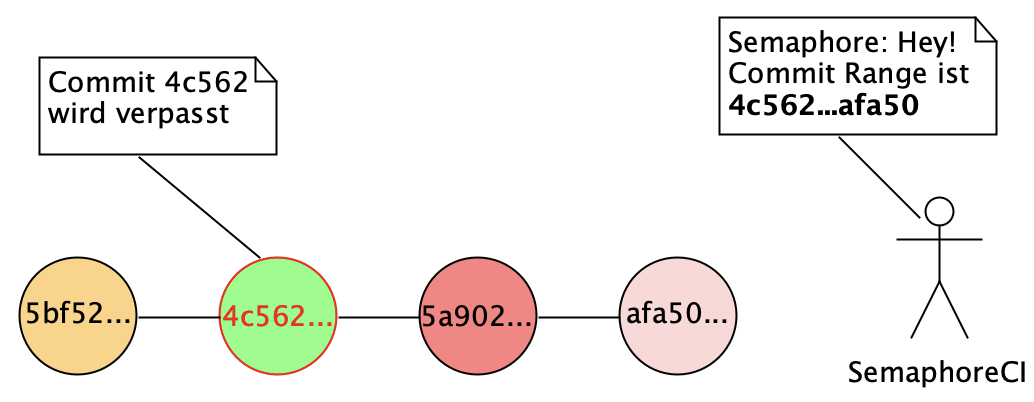
\includegraphics[width=0.8\textwidth]{images/misc/missed_commit_range.png}
  \caption[UMLet Diagramm eines Beispiels für verpasste Commits]{Beispiel für verpasste Commits}
  \label{fig:commit_range}
\end{figure}
Falls aber der erste Commit in der Range fehlt, ist das eher weniger ein Problem, da man nachschauen
kann, welcher der erste, noch nicht releaste, Commit ist und dann die Range manuell eingrenzen kann. \newline
Falls aber der letzte fehlt, kann man das nicht mehr. Und was passiert, falls die History Rebased wird?
Und in anderen Edge-Cases? Falls diese PA ein Produkt liefern will, welches in der Praxis eingesetzt wird,
liefert das aktive Polling eine zusätzliche Schicht Sicherheit, dass die kommunizierten Daten wahrheitsgetreu
sind.

\subsection{Tech-Stack}
Die Entscheidung für den Tech-Stack ist bereits gefallen, da Redmine diesen vorgibt. \newline
Die Datenbank für die CI, sowie das lokale testen wird PostgreSQL sein, da dass der Standard bei der Renuo AG ist.

\subsection{Mockups}
\subsubsection{Bewertungsmatrix}
\begin{center}
    \resizebox{0.75\textwidth}{!}{%
        \begin{tabular}{|c|c|c|c|}
            \hline
            \textbf{Kriterium} & \textbf{Gewichtung} & \textbf{Zwei Listen} & \textbf{Unterlisten} \\ \hline
            Übersichtlichkeit & 40\% & 8 & 7 \\ \hline
            Zuordnung & 50\% & 6 & 10 \\ \hline
            Ästhetik & 10\% & 8 & 9 \\ \hline
            \textbf{Total} & --- & 7 & \textbf{8.7} \\ \hline
        \end{tabular}%
    }
\end{center}

\subsubsection{Entscheidung}
Option zwei, aus Grafik \ref{fig:mockup_sublists}, wurde gewählt, da die Deployments besser zu den Pull Requests
zugeordnet werden können. Der Nachteil ist, dass es sehr schnell sehr unübersichtlich werden kann, doch in der Realität
hat es zu jedem Issue selten mehr als eine Pull Request, weshalb das kein grosses Problem darstellt.
